%%%%%%%%%%%%%%%%%%%%%%%%%%%%%%%%%%%%%%%%%%%%%%%%%%%%%%%%%%%%%
% ISB 2023 Abstract Template
% Created by:   Andrew Pohl
%               Faculty of Kinesiology 
%               University of Calgary
%               github.com/AndyPohlNZ/ISB_AbstractTemplate
%%%%%%%%%%%%%%%%%%%%%%%%%%%%%%%%%%%%%%%%%%%%%%%%%%%%%%%%%%%%%

% Required Packages
\documentclass[11pt]{article}
\usepackage{mathptmx}
\usepackage[utf8]{inputenc}
\usepackage{hyperref}
\usepackage{geometry}
\usepackage{graphicx}
\usepackage{multicol}
\usepackage[singlelinecheck=false]{caption}
\usepackage{titlesec}
\usepackage{etoolbox}

% Set page geometry, section headings and figure environment to the requried defaults
% Do not change!
\geometry{
 a4paper,
 left=15mm,
 right=15mm,
 top=20mm,
 bottom=20mm
 }
\titleformat{\section}{\normalfont\fontsize{11}{11}\bfseries}{\thesection}{11pt}{}
\titlespacing\section{0pt}{11pt plus 0pt minus 0pt}{0pt plus 0pt minus 0pt}
\setcounter{secnumdepth}{0}
\setlength{\parindent}{0cm}
\setlength{\columnsep}{7.5mm}


% figure environment
\newenvironment{Figure}
  {\par\medskip\noindent\minipage{\linewidth}}
  {\endminipage\par\medskip}
\captionsetup[figure]{font=footnotesize, labelfont={bf}, name={Figure}, skip=0pt}

% table environment
\AtBeginEnvironment{tabular}{\fontsize{11pt}{13pt}\selectfont}
\newenvironment{Table}
  {\par\medskip\noindent\minipage{\linewidth}}
  {\endminipage\par\medskip}
\captionsetup[table]{font=footnotesize, labelfont={bf}, name={Table}, skip=0pt}
%  modified title/author/affiliation set up.
\newcommand{\settitle}[1]{\title{\vspace{-1.5cm}\fontsize{11pt}{13pt}\selectfont{\uppercase{\textbf{#1}}} \vspace{-0.5cm}}}
\newcommand{\setauthor}[1]{\author{\vspace{-11pt}\fontsize{11pt}{13pt}\selectfont{{#1}}}}
\newcommand{\setemail}[1]{\fontsize{11pt}{13pt}\selectfont{{Email: #1}}}
\newcommand{\setaffiliations}[2]{\date{\vspace{-11pt}\fontsize{11pt}{13pt}\selectfont{{#1 \\\setemail{{#2}}}}}}
    

% -------- Preliminaries ---------
% Set Abstract title
\settitle{Abstract Submission Guidelines for ISB2023} 
% Set author names, affiliations and contact email.
\setauthor{First Author$^1$, Second Author$^2$, Third Author$^{1,2}$} % Set authors
\setaffiliations{$^1$Department, University / Institute, City, Japan\\ 
    $^2$Department, University / Institute, City, Japan}{isb-jsb2023-ab@congre.co.jp}


% -------- Preliminaries ---------
\begin{document}
\maketitle % Create title
\thispagestyle{empty} % Remove page numbers

\begin{multicols}{2}
\section{INTRODUCTION}
This page contains information about the abstract submission process and represents the template you must use to format your abstract. All abstracts \emph{must} be submitted via the abstract submission system of the congress website by 31 January 2023. All abstracts \emph{must} be submitted as PDF files and must be smaller than 8 MB. You will be notified in mid-March if your abstract is accepted. The conference organizers reserve the right to reject abstracts that do not adhere to this template. 
The body of the manuscript should be divided into the following sections: INTRODUCTION, METHODS, RESULTS, and CONCLUSIONS. The text within each column should be right- and left-justified, without paragraph indentations.

\section{METHODS}
The abstract should be one A4 size page (210 x 297 mm), with two columns of text, justified. The top margin should be 20 mm, while left, right and bottom margins should be 15 mm. Type font is Times New Roman 11 pt, except for the figure/table captions, which should be in size 9 pt. This template is used to format your paper and style the text. All margins, line spaces, and text fonts are prescribed; please do not alter them.
The title (bold caps), authors, and author affiliations should be centered across the top of the page. Use numerical superscripts to distinguish authors who are from different institutions. An email address of the corresponding author must be included. All authors should have made substantial contributions to all of the following: (1) the conception and design of the study, or acquisition of data, or analysis and interpretation of data, (2) drafting the article or revising it critically for important intellectual content, (3) final approval of the version to be submitted.

\section{RESULTS}
Up to one figure and one table (if included) may be incorporated within the document and should be placed immediately after a paragraph and should be referenced parenthetically in the text (Figure \ref{fig:fig1}). Captions should be placed below each figure and above each table. Tables may extend across two columns when needed, in which case they must be placed at the bottom of the page (Table \ref{tab:tab1}). Captions must be legible and placed below each figure, and above each table. Use numbers in square brackets [1,2] to cite references within the text and format references at the end of the abstract as shown on this page.
\begin{Figure}
    \centering
    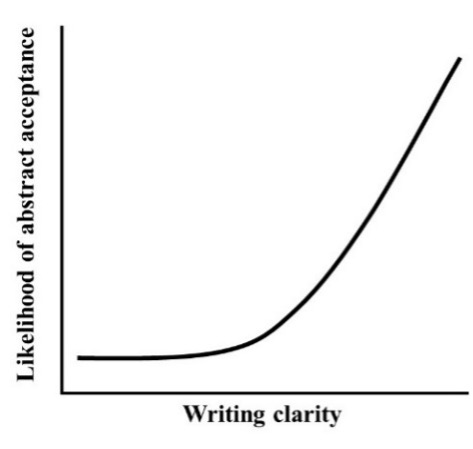
\includegraphics[width=0.75\textwidth]{figures/figure.jpg}
    \captionof{figure}{Likelihood of acceptance as a function of writing clarity. }
    \label{fig:fig1}
\end{Figure}

\section{CONCLUSIONS}
Summarize your main findings and place the findings in the larger context of your field. Use as plain English as possible – avoid jargon. Conclusions should be based directly on the data presented in this study. All questions about the conference should be addressed to \href{mailto:isb-jsb2023-ab@congre.co.jp}{isb-jsb2023-ab@congre.co.jp}.

\section{ACKNOWLEDGEMENTS}
Acknowledgments are optional and may specify research funding and resources including organisation name and reference numbers (if applicable).
\section{REFERENCES}
% For now these are simply manual.  Please seperate references by full line to ensure reference number is displayed.
[1] Hobara H et al. \textit{J Biomech} \textbf{86}: 34-9, 2019.

[2] Kobayashi T et al. \textit{J Biomech} \textbf{130}: 110845, 2022. 
\end{multicols}

% If you have a table which does not fit in a single column it should be placed at the bottom of the abstract and span the page width...
\begin{Table}
    \captionof{table}{Tables that extend across both columns should be placed at the bottom of the abstract.}
    %\centering
    \begin{tabular*}{\textwidth}{@{\extracolsep{\fill}}lcccc}
        \hline
        & Group A & Group B & Effect Size & p-value\\
        \hline
         Variable 1 (Units) & $3.1\pm0.6$ &	$2.4\pm0.7$ & $0.76$ & $p = 0.012$  \\
         Variable 2 (Units)	& $19.2\pm4.2$ & $15.5\pm2.5$ & $1.18$ & $p = 0.001$\\
         \hline
    \end{tabular*}
    \label{tab:tab1}
\end{Table}

\end{document}
